\section{Background}
\label{sec:background}
\subsection{Machine Model}
\label{sec:backgroundonmachinemodel}

In typical system configurations, all memory addresses seen by programs running on modern computers are \emph{virtualized}: the address observed by a running program generally will not correspond directly to the physical location in memory, and may not even correspond to a physical location that \emph{exists} in the machine. Instead, these \emph{virtual} addresses are translated to \emph{physical} addresses that correspond directly to locations in RAM. On most modern architectures, this translation is performed through cooperation of the hardware and OS kernel: while executing an instruction that dereferences a (virtual) address, the CPU's \emph{memory management unit} (\textsc{MMU}) implements an architecture-specific process of \emph{address translation}, resulting in a physical address used to access the cache\footnote{Technically, for performance reasons most caches are indexed with parts of the virtual address, but tagged with the physical data addresses, so cache lookups and address translations can proceed in parallel.} and/or memory-bus.

\begin{figure}
    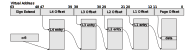
\includegraphics[width=\columnwidth]{pagetables.png}
    \caption{x86-64 page table lookups.}
    \label{fig:pagetables}
\end{figure}

On the x86-64 architecture, the input to the \textsc{MMU}'s address translation is a sparse hierarchical set of tables calle d \emph{page tables} (referring to pages of memory). As Figure \ref{fig:pagetables}\mytodo{cite AMD ref} shows, address translation proceeds by repeatedly taking designated slices of the virtual address and indexing into a table. On x86-64, standard configurations use 4 levels of page tables, labelled levels 4 through 1, with lookups in the level 1 page table resulting in the actual page of physical memory holding the requested data, and the low-order 12 bits being used to index into this page.\footnote{Technically levels 1--3 have designated names originating when there were fewer levels. We omit those names to avoid confusion, and for greater consistency with the recent addition of a 5th level on the most recent processors, where levels 4 and 5 are simply known by their numbers.}  Because address translation traverses a series of tables, the translation process or algorithm is sometimes referred to as a \emph{page-table walk}. While Figure \ref{fig:pagetables} and most of our details are specific to the x86-64 architecture, ARMv8 (a.k.a.\ \texttt{aarch64}), RISC-V, and PowerPC use similar hierarchical page tables for address translation.

The entries of each table are 64 bits wide, but each points to a physical address aligned to 4KB (4096 byte) boundaries, which leaves 12 bits to spare to control a validity bit (called the \emph{present} bit), a read-write bit (which permits write access through the entry if and only if it is set), and a range of additional bits which can be used to control caching, write-through, and more. This paper will only consider the present bit (0), the read-write bit (1), and the accessed bit (5), which is set to 1 by the hardware every time an entry is used, allowing the OS to determine which pieces of memory are used or unused.

The page tables mapping virtual addresses to physical addresses are managed by the OS. Typically each process has its on virtul-to-physical mappings represented by its own page table, which the OS registers with the CPU by storing it in a specific register (\texttt{cr3}) as part of switching to a new process. Using different mappings, which map only disjoint portions of physical memory (with some exceptions in the next section) is how the OS ensures memory isolation between processes.

If an instruction is executed that accesses a virtual address that either has no mapping, or does not have a mapping permitting the kind of access that was performed (e.g., the instruction was a memory write, but the relevant address range was marked read-only in the relevant page table entry), the hardware triggers a \emph{page fault}, transferring control to a \emph{page fault handler} registered with the hardware by the OS, allowing it to take corrective action (described in the next section).

\subsection{Virtual Memory Managers}
\label{sec:backgroundonvmm}
Most OS kernels have a component called a \emph{Virtual Memory Manager} (VMM)\footnote{Not to be confused with Virtual Machine Monitor. In this paper we focus on non-virtualized scenarios, but hardware virtualization extensions for both x86-64 and ARM make use of an additional set of page tables translating what a \emph{guest} considers to be its (virutalized) physical memory to actual physical memory. Our contributions should offer value in this scenario as well.}
which is responsible for setting up page table mappings and for taking action when a page fault occurs. Often, a page fault indicates a bug in a program --- for example, a null pointer dereference crashes a program not because the hardware designates it an error, but because most OSes refuse to map the first 4K worth of virtual addresses, so dereferencing \texttt{NULL} results in a page fault. In such cases, the OS will terminate the program.

In other cases the OS uses page faults to implement specialized functionality and optimizations. A key example of this is (confusingly) called \emph{paging}: saving room in physical RAM by waiting until memory addresses for code are accessed before copying them to RAM (saving process startup time); or copying memory that has not recently been accessed to disk (i.e., in a \emph{swap} file or partition) and marking those page table entries invalid so a future page fault will give the OS the chance to copy the relevant data back into memory when the program tries to access it again.

The key pieces of functionality a VMM must implement itself, or have available in another OS component (depending on design), are
adding a new page mapping (whether the mapped page contains zeros, file data, or swap data), and removing an existing page mapping.
While this initially sounds like relatively modest functionality whose implementation may be complicated by hardware subtleties, a number of more serious complexities must be handled.

For one, virtual addresses may \emph{alias} when more than one is mapped to the same physical memory. This can occur when a process requests it (e.g., via \texttt{mmap} or \texttt{shm\_open} on UNIX-style kernels). It also occurs automatically in most general-purpose kernels: while for normal programs the OS uses the MMU to isolate and abstract physical memory, the kernel's own functionality is often easier to implement if the kernel can directly access memory given its physical address, for example when interacting with hardware devices. For this reason, most kernels contain an \emph{identity map} of all physical memory in a machine. In some cases this is a literal identity map, where for every virtual address $p$, interpreting $p$ as a virtual address instead will map back to $p$ as a physical address. In other cases there is an offset involved, where to access physical address $p$ the kernel can access virtual address $p+\mathit{offset}$. This identity map saves the kernel the performance cost of having to continually add and remove transient mappings simply to briefly access a specific physical memory region. But this coexists with additional virtual addresses (those used by most kernel code and data structures), in a form of virtual address aliasing. Note that virtual address aliasing is both prevalent in general-purpose kernels, and violates the core assumption of most memory models assumed by verified compilers like CompCert, which assume no virtual address aliasing.

Another complicating factor is that portions of page tables can be shared, i.e., trees of page tables can overlap. One common way this used to happen was for one subtree of page tables to map the kernel if linked in appropriately to a higher-level page table, and then to reuse that kernel mapping portion in every process's page tables. This was mostly phased out in the wake of Spectre\mytodo{Colin finish}

These dove-tail with functionality in the OS scheduler, which since it is responsible for dealing with multiple address spaces, must keep track of which virtual addresses are valid (and in what way) in which address spaces, where some virtual addresses are valid in only a single address space (e.g., a code address for a particular usermode process), while others are valid in all address spaces (e.g., kernel data structure pointers). The VMM must maintain some of these assumptions on behalf of the rest of the kernel, for example by guaranteeing that a certain range of virtual addresses (corresponding to the kernel's code and data) are valid in every address space.

\subsection{Modal Logic}
\label{sec:backgroundonmodallogic}
The problem of needing to keep track of things being true in some contexts and not in others is hardly unique to virtual memory management, and is the general insight behind most flavors of modal logic.

Most modal logics use unary operators on propositions to express that a logical claim $P$ is \emph{contingently} true in certain other circumstances, such as in other times~\cite{pnueli1977} or places~\cite{gordon2019modal}. That is, for different modal operators $M$, $M(P)$ may mean that $P$ is true in another time or place (which may be a physical place like another network node~\cite{murphy,gordon2019modal} or a conceptual place like a person's mind~\cite{hintikka1962knowledge}). A unifying concept across any modality is that they behave as applicative functors, typically satisfying (directly, or as a derived law):
\[ (P\rightarrow Q) \rightarrow M(P) \rightarrow M(Q)\]
\mytodo{Ismail, I think this means we have pure intro, $\square P \mathrel{-\ast} [r](\square P)$ if I'm using the right symbol for pure assertions }
Many modalities, so-called \emph{normal} modalities also possess introduction rules of the form $P\rightarrow M(P)$, the classic example being that if $P$ is true, then $P$ is \emph{necessarily} true ($\square P$)

Of particular interest for reasoning about virtual memory are modalities that permit \emph{naming} the alternate circumstances, prominently \emph{hybrid} modal logics~\cite{blackburn1995hybrid,areces2001hybrid}, which come equipped with assertions of the form $@_\ell(P)$ indicating that $P$ is true in the specific alternate circumstance (Kripke world) named by the \emph{nominal} $\ell$.

For our purposes, these are natural candidates to adapt for virtual memory management. We can reinterpret the notion of naming an alternate world slightly more loosely, and instead name \emph{address spaces} by the physical address of the page table root, since these structures are the physical representations of page tables. Thus in this paper we develop the notion that we can represent contingent truth of an assertion via $[r](P)$ indicating that $P$ holds in the address space rooted at physical address $r$.
The typical hybrid modality introduction rule, that $P$ and $\ell$ (indicating the current world is $\ell$) imply $@_\ell(P)$, has a natural analogue: knowing $P$ and that the current address space is $r$ (i.e., that $r$ is the current \texttt{cr3} value) suggests a way to construct $[r](P)$.

A relatively under-explored space of modal logics is the interaction of modal and substructural logics, in particular hybrid-style modalities in substructural logics, which has seen only minimal exploration and no prior application. We develop our ideas in the Iris program logic~\cite{jung2018}, as a result exploring additional subtleties that arise where the modality itself may entail ownership of resources, as well as interactions between our hybrid-style modality and substructural rules.  For example, Iris contains a number of modalities that distribute over separating conjunction, or for which resources can freely move into the modality (e.g., $\blacktriangleright(P)\ast Q \mathrel{-\ast} \blacktriangleright(P\ast Q)$). In our setting some of these rules apply while others do not. For example, in our setting, an assertion that involves no modalities is interpreted as holding in the current (active-on-the-CPU) address space, so clearly cannot move into arbitrary other address spaces --- unless guarded by another address space modality.